\documentclass[11pt,letterpaper]{article}
\usepackage[margin=0.86in]{geometry}
\usepackage[T1]{fontenc}
\usepackage[utf8]{inputenc}
\usepackage{lmodern}
\usepackage{xcolor}
\usepackage{tabularx,booktabs,array,longtable}
\usepackage{enumitem}
\usepackage{hyperref}
\usepackage{fancyhdr}
\usepackage{lastpage}
\usepackage{titlesec}
\usepackage{amsmath,amssymb}
\usepackage{microtype}
\usepackage{needspace}
\usepackage{ragged2e}
\usepackage{graphicx}
\definecolor{navy}{HTML}{19334C}
\definecolor{teal}{HTML}{236B82}
\definecolor{soft}{HTML}{EFF5F7}
\definecolor{muted}{HTML}{52616B}
\hypersetup{colorlinks=true,linkcolor=teal,urlcolor=teal}
\titleformat{\section}{\Large\bfseries\color{navy}}{\thesection.}{0.6em}{}
\titleformat{\subsection}{\large\bfseries\color{navy}}{\thesubsection}{0.6em}{}
\titleformat{\subsubsection}{\normalsize\bfseries\color{navy}}{\thesubsubsection}{0.6em}{}
\titlespacing*{\section}{0pt}{15pt}{6pt}
\titlespacing*{\subsection}{0pt}{10pt}{4pt}
\setlength{\parindent}{0pt}
\setlength{\parskip}{4.5pt}
\setlength{\headheight}{15pt}
\renewcommand{\arraystretch}{1.16}
\setlist[itemize]{topsep=3pt,itemsep=2pt,leftmargin=1.4em}
\setlist[enumerate]{topsep=3pt,itemsep=2pt,leftmargin=1.5em}
\pagestyle{fancy}
\fancyhf{}
\fancyhead[L]{\small\color{muted} Applied Machine Learning \textbar{} Cornell Tech}
\fancyhead[R]{\small\color{muted} Human or AI?}
\fancyfoot[C]{\small\color{muted} Page \thepage\ of \pageref{LastPage}}
\renewcommand{\headrulewidth}{0.3pt}
\newcommand{\placeholder}[1]{\par\noindent\textcolor{teal}{\textit{[Your response: #1]}}\par\vspace{0.3em}}
\newcommand{\figplaceholder}[1]{\par\noindent\fcolorbox{teal}{soft}{\parbox[c][1.15in][c]{0.94\linewidth}{\centering\textcolor{muted}{Insert #1 here}}}\par}
\newcommand{\question}[2]{\needspace{4\baselineskip}\par\addvspace{0.45em}\noindent\textbf{#1}\quad #2\par\nobreak\vspace{0.1em}}
\newcommand{\smallnote}[1]{{\small\color{muted}#1}}
\newcolumntype{Y}{>{\RaggedRight\arraybackslash}X}
\makeatletter\newcommand{\tabinput}[1]{\@@input #1 }\makeatother
\newcommand{\commit}[2]{\href{https://github.com/ZhenmanShen/human-or-ai-submissions/commit/#1}{\texttt{#2}}}
\begin{document}
\thispagestyle{empty}
\vspace*{0.2in}
{\color{teal}\bfseries CORNELL TECH \textbar{} APPLIED MACHINE LEARNING}\par
\vspace{0.15in}
{\Huge\bfseries\color{navy} Human or AI?}\par
\vspace{0.07in}
{\LARGE\color{navy} Kaggle Competition Report --- Classical track}\par
\vspace{0.17in}

\textbf{Report Template: }\href{https://www.overleaf.com/project/6ae1fc85355dcf680137d898/share#f2777b20d3adeeecfac9096f78008e2f8daa0ff4be43de3b}{TEMPLATE}

\textbf{Github Repository Template: }\href{https://github.com/sekhari/human-or-ai-submissions}{REPO}

This track uses only models trained from scratch on the competition data: no pretrained weights, embeddings or tokenizers. Its three headline models are a TF-IDF n-gram logistic regression (C1), 101 hand-crafted stylometric features with LightGBM (C2), and a small Transformer encoder with its own byte-level BPE, trained from random initialisation (C3). All of them run on a laptop CPU, and C3 also on a GPU. They are compared on the same fixed 2,000-row validation split as the team's pretrained-model track.

\vspace{0.06in}
\begin{tabularx}{\linewidth}{@{}>{\bfseries}p{1.58in}Y@{}}
Team / members & [TODO: names and NetIDs] \\
Kaggle team name & [TODO: Kaggle team name] \\
GitHub PR URL & [TODO: PR URL] \\
\end{tabularx}
\vspace{0.06in}
\subsection*{Your data}
\begin{tabularx}{\linewidth}{@{}lrrY@{}}
\toprule
\textbf{File} & \textbf{Rows} & \textbf{Labels} & \textbf{Purpose} \\
\midrule
\texttt{train.csv} & 10,000 & Visible & Supervised model development: 5,000 human (0), 5,000 AI (1) \\
\texttt{unlabeled.csv} & 3,000 & Hidden & Optional input for semi-supervised methods; required experiment \\
\texttt{test.csv} & 3,000 & Hidden & Predict the probability of AI authorship for Kaggle \\
\texttt{train\_starter\_2000.csv} & 2,000 & Visible & Convenient subset of \texttt{train.csv} for quick experiments \\
\bottomrule
\end{tabularx}

\smallnote{The starter data is a subset, not 2,000 additional labeled examples. Passages are approximately 75--350 words, with mean length near 210 words.}

\subsection*{How the test set works}
The test set mixes familiar and unfamiliar writing domains and AI generators, and includes some adversarially modified AI-written passages. You will \emph{not} receive labels, source model names, domain labels, or difficulty memberships for individual test examples. Submit a probability in $[0,1]$ for each test ID, where 1 means AI-generated. Kaggle evaluates submissions using \textbf{area under the ROC curve (AUROC)}. The \textbf{public leaderboard} covers 900 examples (30\%); the \textbf{private leaderboard} covers 2,100 (70\%) and determines the final competition performance score.

\vfill
\newpage
\section{Competition rubric and submission instructions}
\smallnote{Rubric and instructions as in the official template (Kaggle 25, model comparison 15, data size 10, unlabeled data 5, generalization 20, open-ended 15, code/PR 10). Validation protocol used throughout: fixed stratified 2,000-row split of \texttt{train.csv}, seed 20261023 (\texttt{common/val\_ids.csv}).}

\section{Team information and model summary}
\question{Q0.1 [0 points].}{List team members and their main contributions.}
{\raggedright [TODO: names, NetIDs and contributions.] The classical-track framework, the three headline models, the experiments and this draft were produced with Claude Code (see Q6.3); \texttt{classical/CONTRIBUTING.md} describes how teammates add models.\par}

\question{Q0.2 [0 points].}{Summarize your final approach in 3--5 sentences. What is the overall pipeline from raw text to probability?}
The selected classical model is C2. Each raw passage, with its formatting kept, is turned into 101 hand-written stylometric measurements: length and sentence-length statistics, burstiness, type--token and hapax ratios, word repetition, punctuation and function-word rates, readability, adjacent-sentence coherence, blank lines and line structure, and counts of zero-width and homoglyph characters. A LightGBM classifier (63 leaves, learning rate 0.03, 800 trees, chosen by inner cross-validation) maps these features to P(AI). For Kaggle the model is refit on all 10,000 labelled rows. A blend of C1--C3 is 0.0004 better on validation (Q5) but has not been submitted yet.

\question{Q0.3 [0 points].}{Record your final scores (enter private score only once it is revealed).}
\begin{tabularx}{\linewidth}{@{}Yp{1.8in}@{}}\toprule Metric & Your score \\ \midrule Validation AUROC (C2, fixed 2,000 rows) & 0.99831 \\ Kaggle public AUROC & [TODO: pending upload] \\ Kaggle private AUROC & [TODO: after reveal] \\ \bottomrule\end{tabularx}

\newpage
\section{Model comparison and selection (15 points)}
\textbf{Learning goal:} demonstrate sensible representation choices, comparisons of at least three approaches, appropriate hyperparameter selection, and evidence-based selection of the final classifier.

\question{Q1.1 [3 points].}{How did you preprocess and represent the text? Specify tokenization, normalization, word/character features or embeddings, and any feature extraction choices. Why?}
There is no normalisation: case, spacing, line breaks and Unicode are kept, because formatting is informative. Removing C2's layout features costs 0.011 validation AUROC (Q5), and keeping case beats lowercasing for TF-IDF at every C (Q1.3).
\begin{itemize}
\item \textbf{C1} uses sklearn's regex word tokenizer (word 1--2-grams) plus character 2--5-grams within word boundaries. Both are TF-IDF weighted with sublinear term frequency and capped at 300k features each; the vocabulary is fit on the training rows only. Character n-grams capture punctuation habits and sub-word style.
\item \textbf{C2} computes 101 closed-form measurements (Q0.2). Part-of-speech categories are approximated with word lists, so nothing is downloaded.
\item \textbf{C3} uses a 12k byte-level BPE tokenizer trained on the training rows and \texttt{unlabeled.csv} (never validation or test text) and truncates at 512 tokens. Byte-level tokens keep newlines and spaces, which is why they were chosen.
\end{itemize}

\question{Q1.2 [5 points].}{Which \textbf{three or more} modeling approaches did you try? Keep the labeled validation partition fixed across models.}
{\small\begin{tabularx}{\linewidth}{@{}p{1.55in}Yrrr@{}}\toprule
Model & Text representation & Train AUROC & Val. AUROC & Train time \\ \midrule
\tabinput{tables/q12_models.tex}
\bottomrule\end{tabularx}}
\smallnote{Train = the fixed 8,000 rows, Val = the fixed 2,000 rows, seed 20261023. Train time = one fit on the 8,000 rows with the chosen hyperparameters, including feature extraction; CPU = Ryzen 5 9600X. Rows below the line are comparison models.}

\textbf{The six submitted models, both tracks, same validation rows} (\texttt{common/compare\_tracks.py}):

{\small\begin{tabularx}{\linewidth}{@{}Ylrrrlr@{}}\toprule
Model & Track & Train & Val. & Train time & Hardware & Kaggle public \\ \midrule
\tabinput{../../common/tables/six_models.tex}
\bottomrule\end{tabularx}}

\begin{center}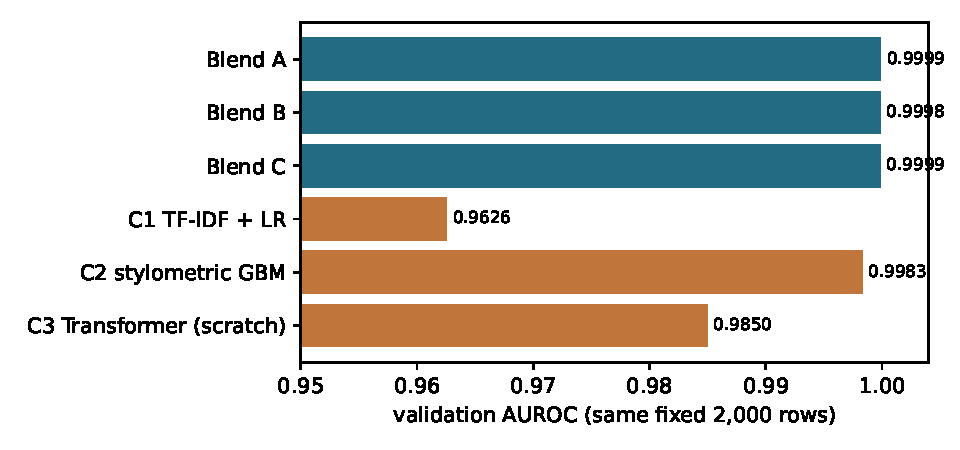
\includegraphics[width=0.49\linewidth]{../../common/figures/six_models.pdf}\hfill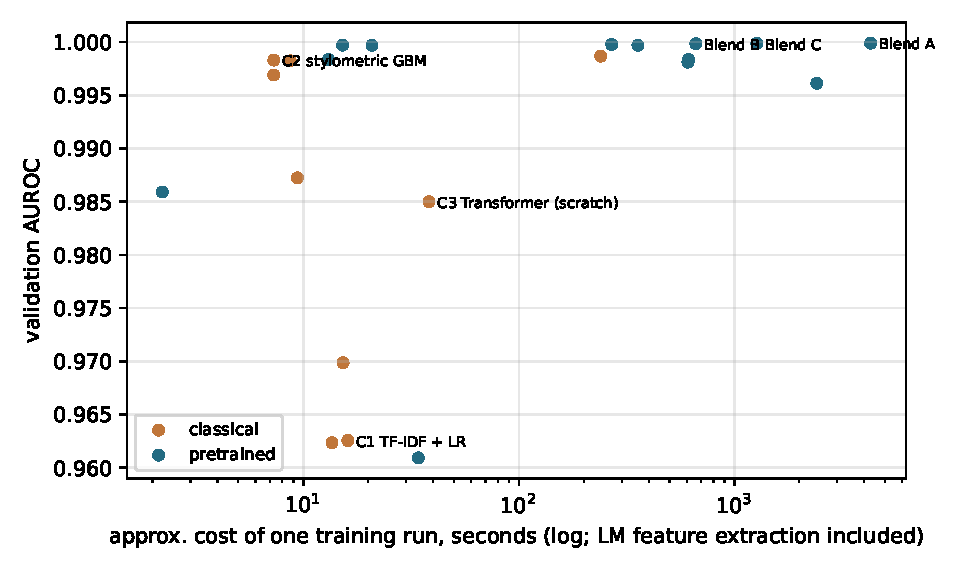
\includegraphics[width=0.49\linewidth]{../../common/figures/cost_vs_auroc.pdf}\end{center}
\smallnote{Pretrained blends: frozen GPT-2 / Qwen2.5 features and fine-tuned RoBERTa/DeBERTa (see the pretrained-track report). Cost axis adds LM feature extraction back for pretrained models.}

\question{Q1.3 [4 points].}{For at least \textbf{two} approaches, which hyperparameters and candidate values did you try? How did you select the final settings without using Kaggle test labels?}
{\small\begin{tabularx}{\linewidth}{@{}p{0.95in}Yp{1.75in}@{}}\toprule Model & Parameters/values searched & Chosen setting \\ \midrule
\tabinput{tables/q13_hpsearch.tex}
\bottomrule\end{tabularx}}

\texttt{train.py} runs every grid point with 5-fold stratified cross-validation inside the 8,000 training rows and keeps the setting with the best mean fold AUROC. It then refits on the 8,000 rows and scores the fixed validation rows once, for reporting only. Validation labels never influence a choice. C3 is not grid-searched (a 5-fold grid would take hours of GPU time); its number of epochs is set by early stopping on a stratified 10\% inner split of its training rows. Observations: TF-IDF prefers weak regularisation (C = 64, the edge of the grid, but +0.0004 over C = 16) and kept case; C2 is flat across all 12 settings (0.9979--0.9981); NB-SVM chose the smallest C, also a grid edge.

\question{Q1.4 [3 points].}{Which approach did you choose for your final submission? Explain using validation performance, computational cost and/or stability. If you later changed the model, explain why.}
We chose C2 (stylometric LightGBM). It is the best of the three headline models on validation (0.99831 vs 0.98500 for C3 and 0.96256 for C1), and it is also the cheapest: a 7-second CPU fit, against 38 s on a GPU for C3. It is stable: inner-CV fold standard deviation is 0.0005, and the score barely moves across the hyperparameter grid. Its learning curve shows it needs little data (Q2). The C1--C3 blend is the only model above it (0.99868), but it costs about 33 times as much to train and puts 90\% of its weight on C2. Whether to spend a Kaggle slot on the blend is [TODO: team decision]. Against the pretrained track, C2 is 0.0016 below blend A on validation. The comparison that matters is Kaggle, where test differs from train in domain and generator. [TODO: public scores of C1--C3 once uploaded.] Full history: Appendix A.

\section{Effect of training data size (10 points)}
\textbf{Learning goal:} understand the effect of the number of labeled examples on fitting and generalization. This is an empirical exercise; no formal sample-complexity theory is required.

\question{Q2.1 [4 points].}{Choose one model configuration. Train it with 500, 1,000, 2,000, 5,000 and 8,000 examples sampled from your 8,000-row training partition. Keep the same validation set and hyperparameters.}
Configuration: C2 with its chosen hyperparameters. Subsets are nested and stratified (seed 20261023); C1 is shown as a contrast.

\begin{tabularx}{\linewidth}{@{}rrrY@{}}\toprule Training rows & Training AUROC & Validation AUROC & Notes (optional) \\ \midrule
\tabinput{tables/q21_curve.tex}
\bottomrule\end{tabularx}
\question{Q2.2 [3 points].}{Insert a plot of training and validation AUROC versus training-set size.}
\begin{center}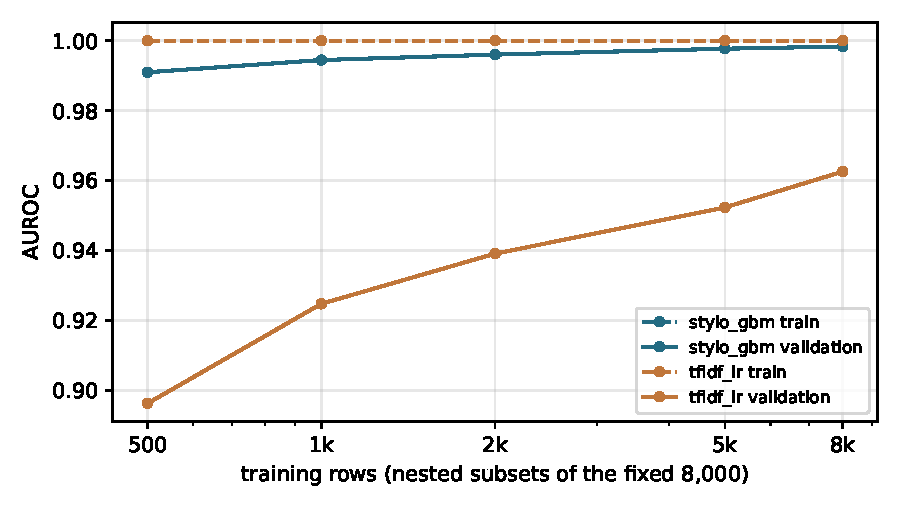
\includegraphics[width=0.72\linewidth]{figures/learning_curve.pdf}\end{center}
\question{Q2.3 [3 points].}{What does the curve suggest about overfitting, underfitting, and the value of more labeled examples?}
Both models reach training AUROC 1.000 at every size: neither underfits, and both overfit in the sense that the training score says nothing about generalisation. Only the validation curve is informative. C2 starts high (0.9910 at 500 rows) and gains about 0.002 per doubling, ending at 0.9983 with the gap to 1.0 still closing slowly. A hundred well-chosen features need few examples to set their thresholds. C1 starts much lower (0.896) and gains about 0.015 per doubling; it is still rising at 8,000 rows, the typical high-variance curve of a model with 600k sparse features. More labels from the same distribution would help C1 noticeably and C2 marginally. Neither curve says anything about test's unseen domains: more \emph{diverse} labels (verse, new generators) would plausibly matter more, but we have no such labelled data to test it.

\section{Learning from unlabeled data (5 points)}
\textbf{Learning goal:} test whether the additional 3,000 unlabeled passages help.
\question{Q3.1 [2 points].}{Describe one method that uses \texttt{unlabeled.csv} (e.g., self-training, confidence-based pseudo-labeling, clustering, or feature learning). How did you prevent validation-label leakage?}
Self-training with the chosen hyperparameters held fixed:
\begin{enumerate}
\item Fit on the 8,000 rows and score \texttt{unlabeled.csv}.
\item Label the 20\% highest-scored passages AI and the 20\% lowest human (1,200 pseudo-labels), add them, and refit.
\item Repeat for 1 or 3 rounds. Each round re-selects from the newest model, starting again from the original 8,000 rows.
\end{enumerate}
Leakage control: the pool is \texttt{unlabeled.csv} only; the validation rows are split off before any fit and never enter training or the pool; and no unlabeled passage is identical to a validation passage (0 matches, checked in \texttt{experiments.py}). C3 also uses \texttt{unlabeled.csv}, but only as tokenizer training text and without labels.
\question{Q3.2 [2 points].}{Compare against a supervised baseline under the same held-out validation protocol.}
\begin{tabularx}{\linewidth}{@{}Yp{1.5in}@{}}\toprule Method & Validation AUROC \\ \midrule
\tabinput{tables/q32_semisup.tex}
\bottomrule\end{tabularx}
\question{Q3.3 [1 point].}{Did it help? Give a concrete, evidence-based explanation (including possible noise in pseudo-labels).}
No. Every change is within $\pm$0.0001 (C1 0.96256 $\to$ 0.96247; C2 0.99831 $\to$ 0.99829 after one round and 0.99835 after three).

The pseudo-labels are near-certain. For C2, every selected passage scored at least 0.99996 (AI) or at most 0.0001 (human); for C1 the cut-offs were 0.985 and 0.020. These are passages the model already classifies correctly, so they add no information, and any wrong ones are confirmed rather than corrected.

{\raggedright \texttt{unlabeled.csv} also has train's mix of forms (1.2\% verse-like passages, against 16.6\% in test; \texttt{common/results/split\_profile.csv}), so it cannot teach the shift that test brings.\par}

\newpage
\section{Generalization and error analysis (20 points)}
\textbf{Learning goal:} characterize how well the selected model generalizes and where it fails. Use \textbf{labeled validation data}; hidden test labels and hidden domain/generator information are unavailable.

\question{Q4.1 [5 points].}{Compare training and validation AUROC for your final selected model. Is there a gap? What explanations are plausible?}
C2 has training AUROC 1.00000 and validation AUROC 0.99831, a gap of 0.0017. At a 0.5 threshold it misclassifies 26 of 2,000 validation passages: 7 false positives and 19 false negatives.

The gap is ordinary overfitting of boosted trees: 800 trees with 63 leaves can memorise 8,000 rows. The inner-CV estimate (0.9981) matches validation, so the gap is stable and not a quirk of this split.

The errors lean towards false negatives, so the model's typical mistake is calling AI text human. For the larger gap to test, the likely cause is distribution shift. half of C2's split gain (50.4\%; blank lines alone 37.5\%, \texttt{results/stylo\_gbm/importances.csv}) comes from the 8 layout features, and test has far more verse (16.6\% vs 1.6\% of training rows), so layout cues may transfer less well. This is a hypothesis.

\question{Q4.2 [5 points].}{Evaluate performance over at least three text-length bins (define the bins), or another observable subgroup available in your data. Explain why you chose the grouping.}
\begin{tabularx}{\linewidth}{@{}Yrr@{}}\toprule Subgroup / bin & Count & Validation AUROC \\ \midrule
\tabinput{tables/q42_subgroups.tex}
\bottomrule\end{tabularx}
\textbf{Groupings.} Word-count bins are $<$150, 150--250 and $>$250 words. Rate features such as type--token ratio and punctuation per word depend on length, so the model might be weaker at the extremes. Line-structure groups are verse ($\ge$4 lines, median $\le$10 words per line, no digits), short-line lists and recipes, and prose. We chose them because C2 leans on layout, and because test is 16.6\% verse.

\textbf{Results.} Long passages are the weakest bin (0.9967 vs 0.9992--0.9993), and short-line lists are slightly weaker than prose (0.9974 vs 0.9985). Verse scores 1.000, but on only 25 rows with 4 AI, which says nothing about test's 498 verse passages.

\question{Q4.3 [5 points].}{Analyze at least \textbf{five false positives and five false negatives} from your held-out validation set. Provide example IDs, predicted probabilities, and short failure hypotheses. Do not paste full passages unless essential.}
{\small\begin{tabularx}{\linewidth}{@{}p{0.5in}p{0.5in}p{0.42in}Y@{}}\toprule ID & Error type & P(AI) & Possible reason \\ \midrule
\tabinput{tables/q43_errors.tex}
\bottomrule\end{tabularx}}
\smallnote{Threshold 0.5 on C2's predicted probability; the five most confident errors of each kind.}

\question{Q4.4 [5 points].}{What recurring failure patterns did you identify, and how might you address one of them? Distinguish observed patterns from speculation.}
\textit{Observed.}
\begin{enumerate}
\item The false negatives are confident (P(AI) $\le$ 0.006) and three of five copy human-looking layout: recipes with one ingredient per line and no blank lines, bullet glyphs, a Wikipedia hatnote with \texttt{[1]} citations. Two of these (1602, 7049) are also errors of the pretrained blend.
\item The false positives are formal, tidy human prose (encyclopedia, an abstract, a polished review) plus one repetitive ramble.
\item Long passages are the weakest length bin.
\end{enumerate}
\textit{Speculation.} C2 learned ``scraped-web layout means human'' because the human training text was scraped and much of the AI text has blank-line paragraphs; AI text written in scraped style breaks that rule. One case (5316, a fluent but factually invented biography) can only be caught by content, not style. \textit{One fix:} the blend's small TF-IDF weight helps (Q5), and a targeted test would augment AI training passages with scraped-web formatting and check whether these false negatives move without hurting validation.

\newpage
\section{Open-ended improvements and insights (15 points)}
\textbf{Learning goal:} propose and test one improvement beyond the required baseline comparisons. This can be simple: a targeted feature change, alternate regularization scheme, ensemble, different representation, augmentation, or training approach. Sophistication alone does not earn credit.

\question{Q5.1 [3 points].}{What specific question or hypothesis motivated your improvement? What weakness or opportunity did you observe?}
The three headline models see different things: C1 sees content n-grams, C2 sees style and layout, and C3 sees token order. Their validation scores are 0.963, 0.998 and 0.985. Hypothesis: they make partly different errors, so a blend weighted on out-of-fold predictions inside the training data beats the best single model (C2). We also asked how much of C2's strength comes from layout, the cue most likely to break on test's verse.

\question{Q5.2 [4 points].}{What exactly did you change? Describe the baseline, the new approach and what you held fixed for a fair comparison.}
\textbf{Baseline:} C2 alone. \textbf{New approach} (\texttt{ensemble\_c123}), computed entirely within the 8,000 training rows:
\begin{enumerate}
\item Each of C1, C2 and C3, with the hyperparameters its own run chose, produces 5-fold out-of-fold predictions on the 8,000 rows.
\item Blend weights come from greedy forward selection with replacement (20 steps) that maximises the out-of-fold AUROC of the weighted mean of percentile ranks.
\item Each member is refit on all 8,000 rows. At prediction time, each member's score is mapped through the CDF of its own out-of-fold scores before weighting.
\end{enumerate}
\textbf{Held fixed:} the training rows, the members' hyperparameters, the seed and the validation rows. Validation is scored once, at the end.

\textbf{Ablations of C2,} with the same hyperparameters and no search: drop the 8 layout features (blank lines, newline rate, paragraph count and length spread, and the line-length statistics), or drop the 9 features added for this track (line structure, zero-width and homoglyph counts).

\question{Q5.3 [4 points].}{What were the measured results?}
{\small\begin{tabularx}{\linewidth}{@{}YrrY@{}}\toprule Configuration & Val. AUROC & Runtime & Relevant difference \\ \midrule
\tabinput{tables/q53_improvement.tex}
\bottomrule\end{tabularx}}
\smallnote{Runtime = one fit on the 8,000 rows (the blend includes its 15 inner-fold fits; C3's ran on an RTX 5070). Blend weights chosen on inner OOF: C2 0.9, C1 0.1, C3 0.0; inner-OOF AUROC 0.99848 for the blend vs 0.99805 for C2 alone.}

\question{Q5.4 [4 points].}{What did you learn? Did the results support the hypothesis? What limits the conclusion, and what would you try next?}
\textbf{The blend: partly supported.} It beats C2 by 0.0004 AUROC and raises TPR at 1\% FPR from 0.983 to 0.990. The inner-OOF weights moved in the same direction before validation was looked at.

The gain comes from C1, not C3. C3 received zero weight: its errors are covered by C2, and its inner-OOF AUROC (0.970) is far lower. A small amount of content signal complements style; a weak sequence model does not.

\textbf{The ablation} confirms the layout concern: without the 8 layout features C2 drops to 0.9872, with TPR at 1\% FPR falling from 0.983 to 0.865. Layout carries a large share of what C2 knows. The 9 features added for this track barely matter (0.0001), because blank lines were already in the base set and adversarial characters appear in only 2 validation passages.

\textbf{Limits:} a 0.0004 difference on 2,000 rows is within noise (we did not bootstrap it), and in-distribution validation cannot show whether layout reliance hurts on test.

\textbf{Next:} bootstrap confidence intervals for the blend's gain; a layout-free C2 variant judged by Kaggle rather than validation; and the formatting augmentation from Q4.4.

\section{Code submission, reproducibility and AI assistance (10 points)}
\textbf{Submission format:} Submit a \textbf{GitHub PR URL} against the course repository. We will inspect the final code and its development history, not just the final snapshot. Do not squash away meaningful intermediate commits before review. Template \href{https://github.com/sekhari/human-or-ai-submissions}{here}.

\question{Q6.1 [5 points].}{Provide the PR URL, the entrypoint for training/evaluation, and the command used to generate \texttt{submission.csv}. State dependencies and random seeds.}
PR: [TODO: PR URL]. Code: \texttt{submissions/<team>/classical/}. Python 3.12 with \texttt{pip install -r requirements.txt} (numpy, pandas, scikit-learn, LightGBM, PyYAML, matplotlib; torch and tokenizers for C3 only). Put the Kaggle CSVs in \texttt{submissions/<team>/data/} or pass \texttt{--data-dir}.
{\footnotesize\begin{verbatim}
python ../common/make_split.py              # verifies the shared split
python train.py --model stylo_gbm           # search, fit on 8,000, score 2,000
python train.py --model stylo_gbm --final   # refit on 10,000 -> kaggle_submissions/
python predict.py --model stylo_gbm --out submission.csv   # from artifacts/
python experiments.py curve                 # also: semisup, errors (Q2-Q4)
python report_tables.py                     # reports/tables, reports/figures
\end{verbatim}}
{\raggedright Seed 20261023 for the split, the CV folds and every model. \texttt{predict.py} re-creates the \texttt{--final} file exactly (max $|\Delta| = 0$, checked for the template model and C3). C3 trains on a GPU in bf16, so a rerun on different hardware can differ slightly.\par}

\question{Q6.2 [3 points].}{Give two or three examples of changes you made during development. Link to relevant commits or PR discussion and briefly explain what the experiments taught you.}
\begin{itemize}
\item \commit{25e13767d61438179159ac80483685b2ae4cf0ce}{25e1376}: TF-IDF grid. Keeping case beats lowercasing at every C (+0.005), so capitalisation habits carry signal. We kept all formatting in the other models too.
\item \commit{345aaab6ff162b0dd75461b219afda13866aed63}{345aaab}: Transformer trained from scratch. Inner-split AUROC peaks at epochs 6--7 and then falls while training loss keeps dropping. With 7,200 passages a 6.4M-parameter model overfits within a few epochs, and early stopping on an inner split (not the validation set) is essential.
\item \commit{6fb8406709d375571d760b4d23b11a131c61c44e}{6fb8406} and \commit{11856a37a75eab0f610fdfb2d9ddff0ae7bbefab}{11856a3}: the layout ablation ($-$0.011) and the C1--C3 blend (weights 0.9 / 0.1 / 0). The style model's strength is partly layout, and the cheap n-gram model complements it better than the Transformer does.
\end{itemize}

\question{Q6.3 [2 points].}{How did you use AI tools (such as Claude, ChatGPT or Copilot) for code, debugging, analysis or writing? What did you verify or modify yourself?}
[TODO: team to edit.] Claude Code (Anthropic) wrote the classical framework (\texttt{train.py}, \texttt{predict.py}, the model plug-in interface), the models, the experiment scripts and this draft, and ran the experiments on our machines. The stylometric feature code was ported from our own earlier research repository. Every table number is generated from the committed results files by \texttt{report\_tables.py}. [TODO: what the team verified or changed themselves.] No pretrained weights, embeddings or tokenizers are used anywhere in this track; the only learned tokenizer is trained here on training and unlabeled text. No external LLM API labelled or scored test passages, and no hidden labels were retrieved.

\textbf{AI policy.} You may use AI assistants for coding, debugging, explanations, brainstorming, and editing. We expect each team to exercise its own judgment, run experiments, check outputs, and understand its submitted approach. Sending the entire assignment to an AI tool and submitting its unverified output without meaningful involvement does not satisfy the objectives of this project. We will use the PR history, reproducible experiments and report together as evidence of engagement. \emph{Commit counts and the presence of AI-generated code are not themselves grading criteria.} Do not fabricate results or retrieve hidden test labels.

\section*{Final submission checklist}
\begin{itemize}[label=$\square$]
\item Final probabilities submitted to Kaggle for every \texttt{test.csv} ID.
\item Completed report, with all required answers, tables, figures and sources, submitted as PDF.
\item GitHub PR linked on the report title page and in the course submission portal.
\item Code and dependencies recreate final predictions (within reasonable numerical tolerance).
\item Relevant experiments and seed/configuration details are recorded.
\item AI-use disclosure is complete; hidden labels were not retrieved externally.
\end{itemize}

\appendix
\section*{Appendix A. Submission and testing history}
Generated from \texttt{submission\_log.csv} (also \texttt{SUBMISSIONS.md}); every model validated on the fixed split, both tracks. ``not submitted'' = tested only; ``pending upload'' = file written, score not yet recorded.

{\footnotesize\begin{longtable}{@{}llp{1.7in}lrll@{}}\toprule
Date & Track & Model & Commit & Val AUROC & Kaggle public & Private \\ \midrule\endhead
\tabinput{tables/appendix_submissions.tex}
\bottomrule\end{longtable}}

\end{document}
